\chapter{Related Work}\label{ch:related-work}

As we discussed in~\Cref{ch:introduction}, to get the easily interpretable graph, its drawing should minimise the number of crossings. The first algorithms, designed to do so programmatically, were designed to recognise planar graphs, and construct a drawing for those who admit such. The first linear-time algorithm for doing so was introduced as early as~\citeyear{linear-p} by \citeauthor{linear-p}~\cite{linear-p}. In this chapter we discuss studies that address the recognition problem for almost planar graphs.

\section{Difficulty of dealing with beyond-planar graphs}

Most relaxations of strict planarity dramatically increase the complexity of recognising such graphs. So, the general problem of minimising edge crossings in a graph drawing was known to be computationally intractable already in~\citeyear{cr_NPC} when \citeauthor{cr_NPC}~\cite{cr_NPC} demonstrated that the \textsc{Crossing Number} problem, where the task is to check whether a given graph can be drawn with at most \(k\) crossings, is NP-hard. Their proof relies on a reduction from the \textsc{Optimal Linear Arrangement} problem, which is known to be NP-hard.

Minimising the number of local crossings is also hard. \citeauthor{1p-NPH}~\cite{1p-NPH} showed that testing \(1\)-planarity, that is, recognising whether a graph can be drawn with at most one crossing per edge, is NP-hard. Later, \citeauthor{one-edge-NPH}~\cite{one-edge-NPH} showed that testing~\(1\)-planarity is NP-hard even for near-planar graphs, that is, graphs that can be obtained from planar graphs by adding a single edge.

\begin{figure}[tbh]
    \centering
    \captionsetup{subrefformat=parens}
    \subfloat[\(1\)-planar drawing]{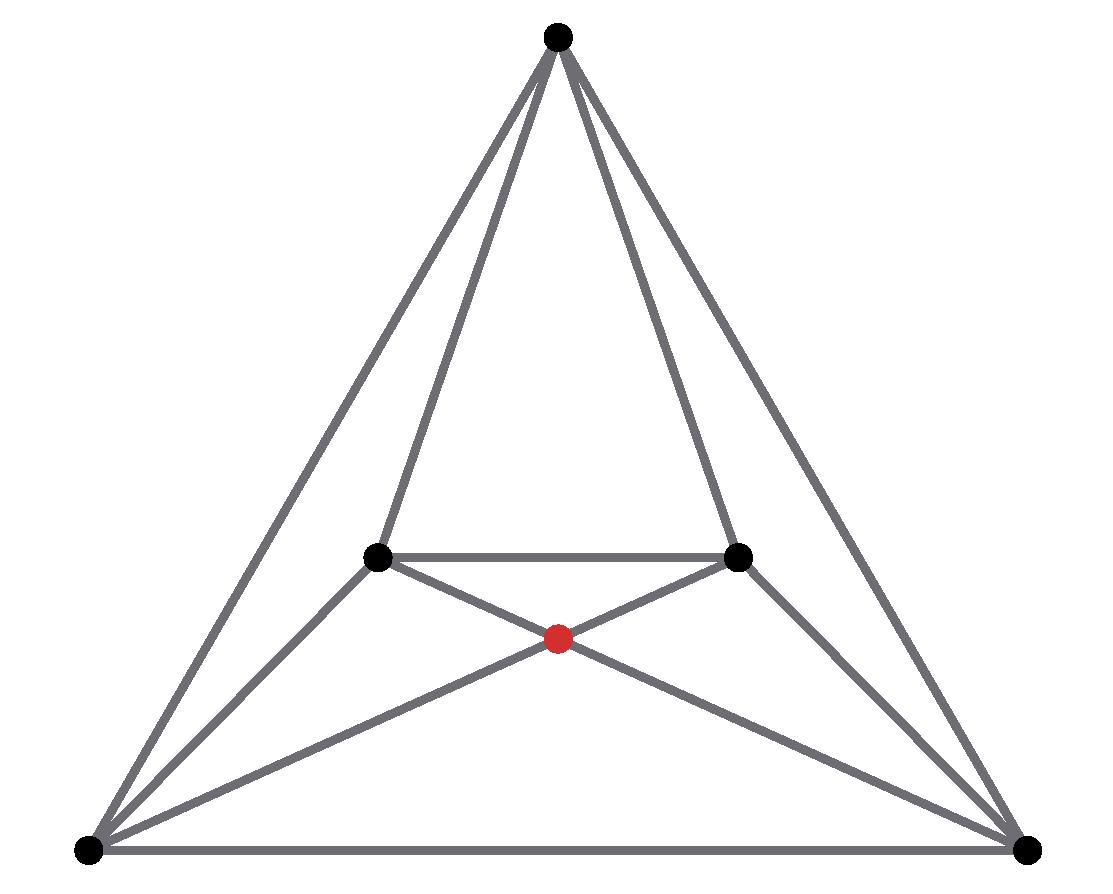
\includegraphics[width=0.3\textwidth]{k5_1planar}\label{fig:k5:1-planar}}
    \subfloat[Outer \(2\)-planar drawing]{
\includegraphics[width=0.3\textwidth]{k5_outer2planar}\label{fig:k5:o2p}}
    \caption{Drawing of \(K_5\) \subref{fig:k5:1-planar}~non-restricted and \subref{fig:k5:o2p}~restricted to a circular setting.}
    \label{fig:figure}
\end{figure}

Given the complexity of recognising \(k\)-planarity, researchers have considered exploring more restrictive settings, hoping that the imposed limitations could simplify the recognition. One of the considered restrictions is a circular setting that requires the vertices to be placed on a circle and the edges to be drawn as straight lines. This restriction gives rise to the \emph{circular local crossing number} of a graph, which we study in this thesis. The graphs whose circular crossing number is bounded by \(k\) are called \emph{outer \(k\)-planar} graphs. For example, \(K_5\), the complete graph with five vertices, is known to be the smallest non-planar graph. It can be drawn with a single crossing, hence it is \(1\)-planar (see~\Cref{fig:k5:1-planar}). When insisting on the circular setting, however, every second edge receives two crossings, hence \(K_5\) is outer \(2\)-planar (see~\Cref{fig:k5:o2p}).


\section{Efficient recognition of some outer \texorpdfstring{\(k\)}{k}-planar graphs}

Although the recognition problem for outer \(k\)-planar graphs is NP-hard if \(k\) is a part of the input, efficient algorithms have been developed for any constant value of \(k\).

For \(k = 0\), the recognition task simplifies to an outerplanarity test. Recognition can be accomplished by augmenting the graph with a new vertex connected to all original vertices and testing whether the resulting graph is planar. An alternative approach, described in~\cite{linear-op}, introduces the concept of~\(2\)-reducible graphs, which are totally disconnected or can be made totally disconnected by repeated deletion of edges adjacent to a vertex with a degree at most two. The proposed outerplanarity test is based on an algorithm for testing~\(2\)-reducibility.

In the case of \(k = 1\), two research groups independently presented linear-time algorithms~\cite{linear-o1p_, linear-o1p}. Both algorithms use the SPQR decomposition of a graph for the test. Notably, the latter solution extends the graph to a maximal outer~\(1\)-planar configuration if such a drawing exists, unlike the former, which employs a bottom-up strategy which does not require any transformations of the original graph.

Considering a special case of this problem, \citeauthor{linear-full-o2p}~\cite{linear-full-o2p} proposed a linear-time algorithm for recognising full outer~\(2\)-planar graphs. An outer \(k\)-planar drawing is \emph{full} if no crossings lie on the boundary of the outer face. Later, \citeauthor{linear-full-okp}~\cite{linear-full-okp} extended their result by introducing an algorithm for recognising full outer \(k\)-planar graphs for every \(k\). Their algorithm runs in \(O(f(k) \cdot n)\) time, where \(f\) is a computable function.

For the general version of the problem and values of \(k > 1\), no research was conducted until recently when a group of researchers proposed an algorithm for the general case, which we discuss in the~\Cref{sec:recognising-general-outer-(k)-planar-graphs}.


\section{Recognising general outer \texorpdfstring{\(k\)}{k}-planar graphs}\label{sec:recognising-general-outer-(k)-planar-graphs}

For a given outer \(k\)-planar drawing of a graph, \citeauthor{triangulations}~\cite{triangulations} proposed a method for constructing a triangulation with the property that each edge of the triangulation is crossed by at most \(k\) edges of the graph drawing. Since the edges of the triangulation do not necessarily belong to the original graph, they are termed \emph{links} to distinguish them from the original graph edges. The construction is done recursively.

Initially, the algorithm selects an edge on the outer face and labels it as the active link. At each recursive step, the active link partitions the graph into two regions: a left part already triangulated and a right part not yet explored. The objective of each step is to triangulate the right portion. To achieve this, a splitting vertex is chosen within the right region, dividing it into two smaller subregions. The splitting vertex is selected so that the two new links, connecting the split vertex with the endpoints of the active link, are each intersected by at most \(k\) edges, which allows including them into the triangulation. The algorithm then recurses, treating each of these newly formed links as the active one.

Later, \citeauthor{okp}~\cite{okp} extended this approach to address the recognition problem for outer \(k\)-planar graphs. In contrast to the triangulation task, where the drawing is provided, the recognition problem requires determining whether a given graph admits an outer \(k\)-planar drawing. Although the core idea remains analogous, the absence of a drawing requires the exploration of all possible configurations. Here, each recursive step verifies whether the unexplored right portion of the graph can be drawn as an outer \(k\)-planar graph that is compatible with the left part.

Moreover, instead of relying on recursion, the method utilises a dynamic programming approach. This framework combines solutions of smaller subproblems retrieved from a table to solve larger ones. To populate this table, the algorithm iterates over all possible configurations corresponding to different recursion steps. Several parameters characterise each such configuration. The first parameter is the active link~--~a pair of vertices that divides the graph into a left and a right region. The second parameter is a set of vertices in the right part, which is not uniquely determined as in the triangulation case. Additionally, the configuration depends on the order in which edges intersect the active link and the number of intersections on the right side for each one of them. These parameters are used to ensure that the drawing of the right part is compatible with the left part. For each configuration, the algorithm considers all possible ways to split the right region further. For each of them, the method checks whether these splits are compatible with each other and the left part of the drawing.

Using the restriction on the number of edges crossing each link, the authors demonstrated that for a fixed \(k\), the number of possible right subgraphs grows only polynomially with respect to the size of the graph. They proceeded by arguing that the overall time complexity of the algorithm is~\(2^{O(k \log k)}n^{3k + O(1)}\), showing that the algorithm is efficient for any fixed parameter \(k\). This indicates that this problem belongs to the XP class~--~a class of problems that admit such ``slicewise polynomial'' algorithms.


\section{Our contribution}

A common drawback of the methods described above is the lack of practical validation. Although these algorithms have been analysed and discussed in a theoretical context, they have not been implemented or tested empirically. We address this gap by implementing the most recent recognition algorithm and introducing two alternative approaches based on Integer Linear Programming (ILP) and Satisfiability (SAT) formulations. While it is NP-hard to solve the general integer linear programming problem or to find a satisfying truth assignment for general Boolean formulas, there are very advanced solvers for such formulations that allow us to find exact solutions for small- to medium-sized instances within an acceptable amount of time. We evaluate the performance and efficiency of these methods, demonstrating their practical applicability and their limitations.
